\section{Uniform Distribution Dataset}

\subsection{Part A: Developing Hypotheses}
Identify and collect a real-world dataset that you hypothesize follows a Uniform distribution. Please be clear about the reasoning behind your hypothesis and be specific about the source of the dataset.\\
-----\\
For this example, we sourced a dataset of 20-sided (d20) die rolls \hyperlink{https://www.kaggle.com/datasets/devocorum/d20-rolls}{from Kaggle}. The dataset contains the outcomes of 145 rolls of a single, unweighted d20. We hypothesize that this data follows a Uniform distribution because an unweighted die ought to have an equal probability of landing on any of its faces.\\

That would make repeated d20 rolls a clear example of a discrete uniform distribution, where all possible values in its range are equally massed. The probability mass function for a discrete uniform distribution from \( a \) to \( b \) (inclusive) is given by:\\

$$
P(X = x) = \frac{1}{b - a + 1}, \quad \text{for } x \in \{a, a+1, \ldots, b\}
$$

where $ a $ is 1 and $ b $ is 20, so each face of the die ought to have a probability of around:\\
\[
P(X = x) = \frac{1}{20} = 0.05
\]

Because the d20 has a finite outcome space and possesses a notion of fairness, we expect the Uniform distribution to be the most appropriate model for representing this sample. It specifies exactly the parameters necessary to characterize this environment; nothing more imposed. The die doesn't not possess notions of general behavior or extreme values nor does it possess a unique spread of mass within different ranges of outcomes; it simply traverses the outcome space freely, bounded only by the values it can take on.\\
\newpage

\subsection{Part B: Fitting Distributions}
For this exercise, we will call each of the four different theoretical distributions (normal, uniform, power law, exponential) a ``model". Fit the dataset (i.e., estimate the model parameters) against each model (not just the one you hypothesized) using maximum likelihood estimation (or using any technique you think is appropriate; make sure to comment on the validity of your approach). This should result in a total of \textbf{4 parameter sets}. Report the estimated parameters in the following tabular format:

\begin{center}
\begin{tabular}{|c|c|c|c|c|c|}
\hline
& & \multicolumn{4}{c|}{{\bf{\em{Model}}}}\\
\hline
{{\bf{\em{Dataset}}}} & {\bf{\em{\# Observations}}} &\textbf{Normal}& \textbf{Uniform} & \textbf{Power law} & \textbf{Exponential} \\
\hline
\textbf{Dataset 2} & $n_2$ & $\mu_2, \sigma_2$ & $a_2, b_2$ & $\alpha_2, x_{\min_2}$ & $\lambda_2$ \\
\hline
\end{tabular}
\end{center}

Be sure to show the code you used to arrive at your final estimates clearly.\\
-----\\
Below are the tabulated parameter estimates for this dataset (for the full tabulation described in the original assignment TeX, see Appendix). The code in Fig. 1 was also used to arrive at our final parameter estimates for this dataset, here is the same implementation below for convenience:\\

\begin{verbatim}
def dists_fit(input_csv: str) -> tuple:
    """
    Fits the obs dataset to each model using MLE.

    :param input_csv: Path to input data to fit paramater(s) to
    :type input_csv: str
    """
    obs = pd.read_csv(input_csv).iloc[:, 0].to_numpy()

    mu = np.mean(obs)
    std = np.sqrt(np.sum((obs - mu) ** 2) / len(obs))

    a, b = obs.min(), obs.max()

    alpha = 1 + len(obs) / np.sum(np.log(obs / a))

    lamb = 1 / np.mean(obs)

    return (mu, std, a, b, alpha, lamb)
\end{verbatim}

\vspace{4pt}

\begin{center}
\begin{tabular}{|c|c|c|c|c|c|}
\hline
& & \multicolumn{4}{c|}{{\bf{\em{Model}}}}\\
\hline
{{\bf{\em{Dataset}}}} & {\bf{\em{\# Observations}}} &\textbf{Normal}& \textbf{Uniform} & \textbf{Power law} & \textbf{Exponential} \\
\hline
\textbf{D20 Rolls} & 145 & 11.117, 6.055 & 1, 20 & 1.459, 1 & 0.090 \\
\hline
\end{tabular}
\end{center}

\begin{center}
\textbf{Figure 7:} Parameter estimates for each model on D20 Rolls dataset.
\end{center}
\newpage

\subsection{Part C: Comparing Real and Synthetic Data}

For each fitted distribution (there will be 4 of them for this dataset, each corresponding to a different model), generate a synthetic sample of data points equal to the sample size of the real dataset using the respective model parameters you inferred from the real dataset.\\

Compare the real vs. synthetic data distributions using methods you think are the most appropriate, including visualizations. So, for this dataset, we compare the original dataset to four synthetic datasets, all with equal number of observations, but each synthetic dataset is generated using a different model.\\

For this dataset, identify the synthetic dataset (which corresponds to a model) that is most similar to the original data in terms of its distribution.\\

Now revisit your initial hypothesis. For this dataset: Did the dataset behave as expected, or was another model (assumed distribution) a better fit to the dataset? Reflect on why the observed results may differ from your expectations.\\
-----\\
To assess the synthetic data versus the real sample given our Uniform hypothesis, we need an understanding of how evenly distributed the probability mass is of the real sample and each of the model samples. That makes a histogram plot sound very appealing, however some of the other models, namely the exponential model and especially the power law model, fit toward very infrequent extreme values, which make it rather hard to visualize bins of die roll values in this way. Additionally, the Normal model possesses the unique quality of fitting toward a symmetric distribution, allowing for negative roles at the extremes of its distribution. That being said, we first take a look at their K-S statistics tabulated below:

\begin{center}
\begin{tabular}{|c|c|c|c|}
\hline
\textbf{Distribution} & \textbf{K-S Statistic} & \textbf{p-value} & \textbf{Significant} \\
\hline
Normal & 0.11 & 0.341 & No \\
\hline
Uniform & 0.12 & 0.273 & No \\
\hline
Power Law & 0.30 & 5.00 $\times 10^{-6}$ & Yes \\
\hline
Exponential & 0.21 & 0.004 & Yes \\
\hline
\end{tabular}
\end{center}

\begin{center}
\textbf{Figure 8:} Kolmogorov-Smirnov test results between D20 Die Rolls dataset and synthetic samples.
\end{center}

Interestingly enough, the K-S statistic accompanied with p-values shows that the Power Law model and the Exponential model are unsuitable for representing the real data die rolls, showing relatively higher disagreement that is almost certainly significant in nature, however the representative ability of the Normal and Uniform distribution appear quite similar from this test despite the fact that the Gaussian can and will sometimes sample values outside of the outcome space.\\

We now plot for our two most representative models the aforementioned histogram, without any worries of single extremes obfuscating the entire visual:

\begin{center}
  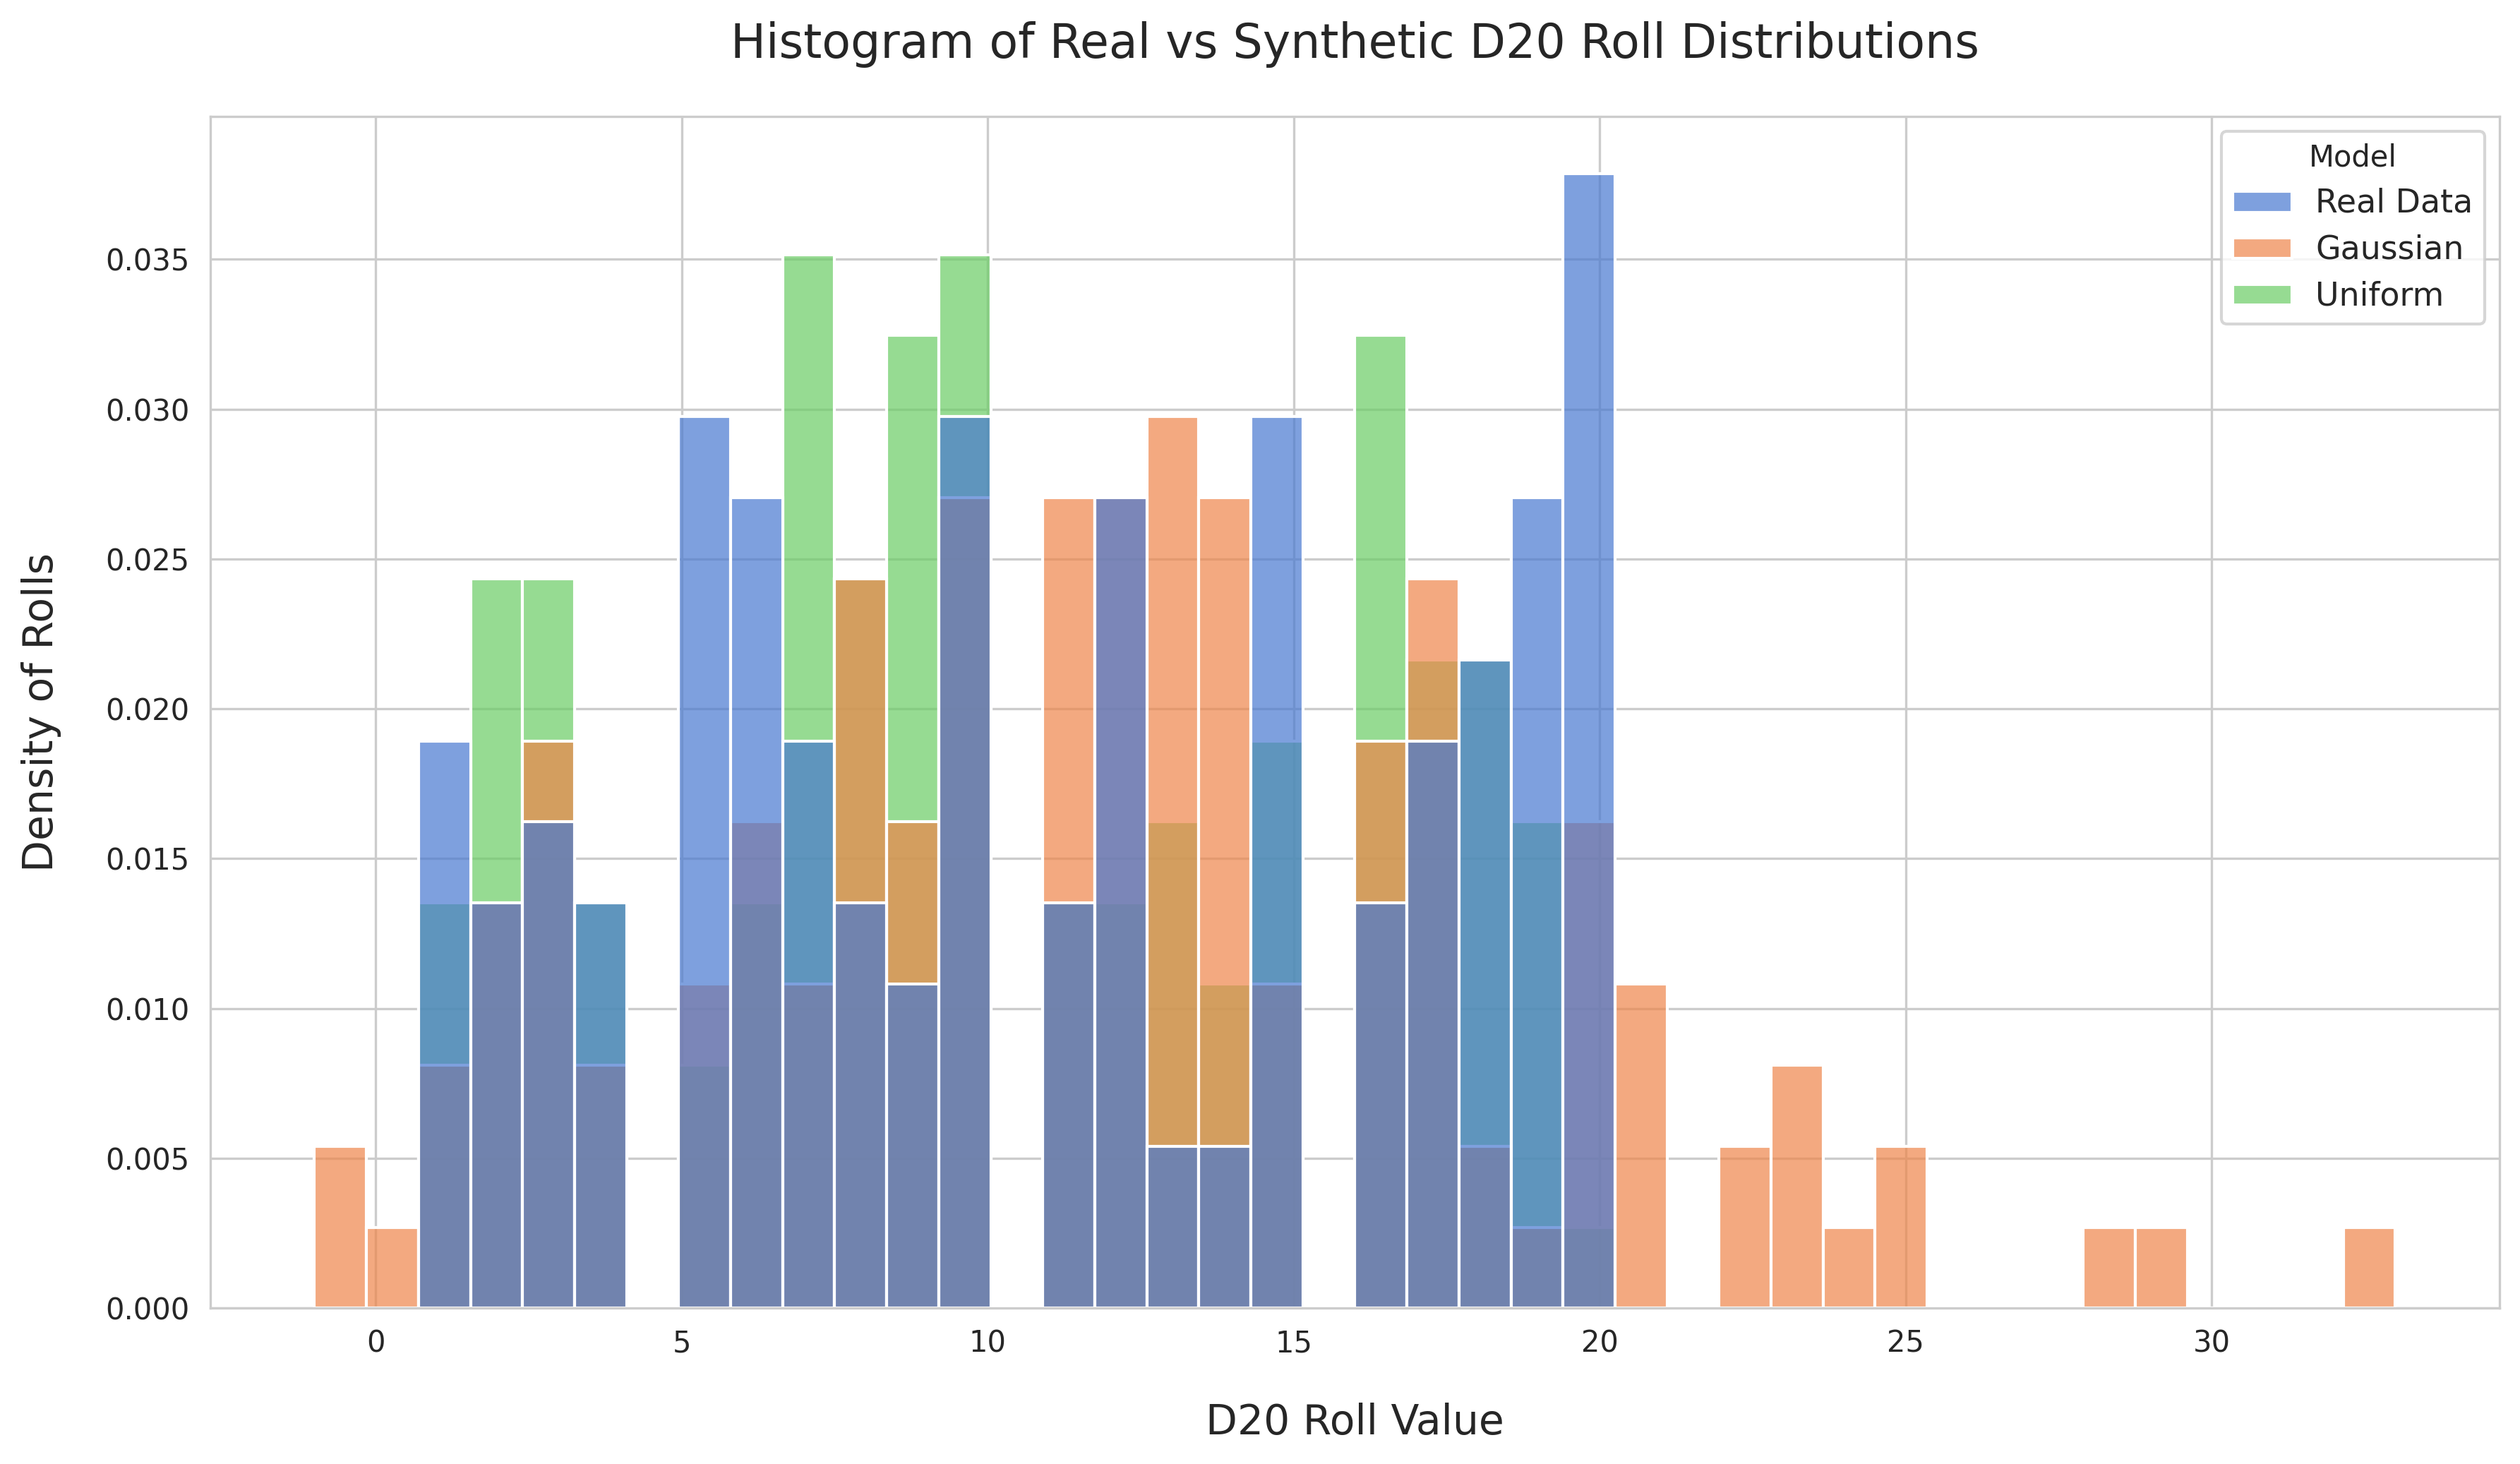
\includegraphics[width=0.90\textwidth]{figures/uniform/histogram.png}
  
  \textbf{Figure 9:} Histogram of Real vs Synthetic Distributions on D20 Die Rolls dataset.
\end{center}

It is immediately obvious from this plot that the Normal distribution is not as well-representative of the real sample toward extreme values, where the underlying assumptions of the uniform model regarding outcome space become relevant. The Uniform distribution mirrors the sporadic distribution of mass as the real sample set within the realms of possibilities for the die.\\

We can make a confident claim that the data sample produced by the Uniform model best represents the original data from its distribution. This confirms our hypothesis and the dataset behaved as we had expected; unweighted dice ought to be uniform in outcome.
